%TITULO------------------------------------------------------------------------

%==============================================================================
\chapter{Modelagem de Conversores Conectados à Rede Elétrica via Filtro LCL}
\label{modelagem}
%==============================================================================

	%intro temporária, melhorar
	Este capítulo apresenta a modelagem de conversores de potência conectados à rede
    elétrica via filtro LCL. São apresentados modelos dinâmicos e em espaço de
    estados, bem como em coordenadas $\alpha \beta 0$ \cite{ref:JORGE} e em
    função de transferência, considerando a corrente $i_C$ e a tensão $v_C$
    do capacitor como variável intermediária. Modelos em tempo discreto são
    desenvolvidos, levando em conta o impacto do atraso de transporte da
    implementação digital.


\section{Modelo em Espaço de Estados - Coordenadas \emph{abc}}

    Considere um conversor trifásico conectado à rede elétrica via filtro LCL
    conforme a Fig.~\ref{fig:LCL_topologia_2}. Considere ainda a rede elétrica
    como sendo uma fonte de tensão trifásica alternada equilibrada com uma
    impedância série equivalente com característica indutiva.

    \begin{figure}[htb]
        \centering{
            %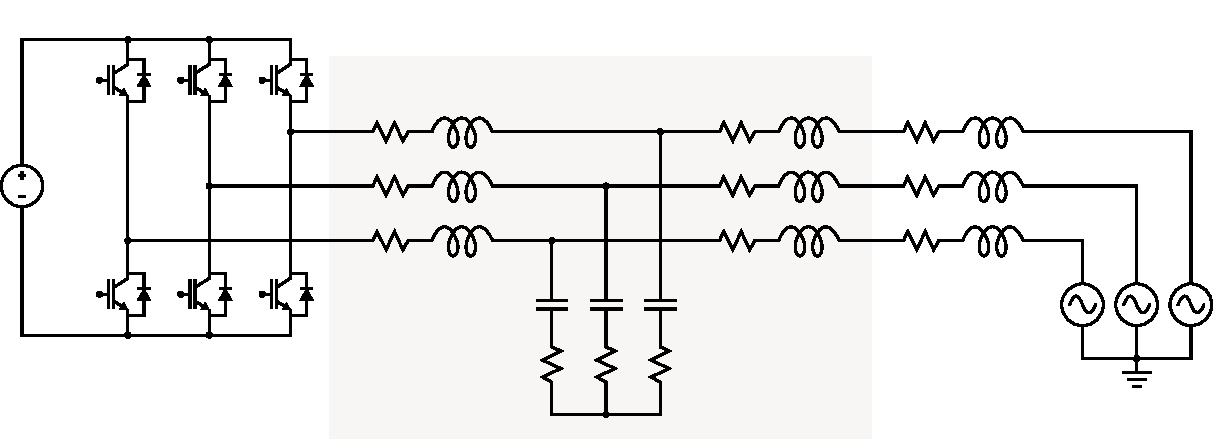
\includegraphics[width=0.9\textwidth]{img/topologia}}
            \def\svgwidth{\textwidth}
            \input{./img/topologia.pdf_tex}}
        \renewcommand\figurename{Fig.}
        \caption{Topologia do filtro LCL.}
        \label{fig:LCL_topologia_2}
    \end{figure}

    A partir das leis de Kirchhoff pode-se obter:
    %
    \begin{equation}
        u_{ab}(t) = R_1 i_{a1}(t) + L_1 \frac{d}{dt} i_{a1}(t) + v_{an}(t)
            - v_{bn}(t) - L_1 \frac{d}{dt} i_{b1}(t) - R_1 i_{b1}(t) \text{,}
    \end{equation}
    %
    \begin{equation}
        u_{bc}(t) = R_1 i_{b1}(t) + L_1 \frac{d}{dt} i_{b1}(t) + v_{bn}(t)
            - v_{cn}(t) - L_1 \frac{d}{dt} i_{c1}(t) - R_1 i_{c1}(t) \text{,}
    \end{equation}
    %
    \begin{equation}
        i_{a1}(t) + i_{b1}(t) + i_{c1}(t) = 0 \implies \frac{d}{dt} i_{a1}(t)
            + \frac{d}{dt} i_{b1}(t) + \frac{d}{dt} i_{c1}(t) = 0 \text{.}
    \end{equation}

    Além disso, das tensões nos capacitores:
    %
    \begin{equation}
        C \frac{d}{dt} v_{an}(t) = i_{a1}(t) - i_{a2}(t) \text{,}
    \end{equation}
    %
    \begin{equation}
        C \frac{d}{dt} v_{bn}(t) = i_{b1}(t) - i_{b2}(t) \text{,}
    \end{equation}
    %
    \begin{equation}
        C \frac{d}{dt} v_{an}(t) + C \frac{d}{dt} v_{bn}(t) +
            C \frac{d}{dt} v_{cn}(t) = 0 \text{.}
    \end{equation}

    E das correntes do lado da rede:
    %
    \begin{equation}
        v_{ab}(t) = R_2 i_{a2}(t) + L_2 \frac{d}{dt} i_{a2}(t) + v_a(t) - v_b(t)
            - L_2 \frac{d}{dt} i_{b2}(t) - R_2 i_{b2}(t) \text{,}
    \end{equation}
    %
    \begin{equation}
        v_{bc}(t) = R_2 i_{b2}(t) + L_2 \frac{d}{dt} i_{b2}(t) + v_b(t) - v_c(t)
            - L_2 \frac{d}{dt} i_{c2}(t) - R_2 i_{c2}(t) \text{,}
    \end{equation}
    %
    \begin{equation}
        i_{a2}(t) + i_{b2}(t) + i_{c2}(t) = 0 \implies \frac{d}{dt} i_{a2}(t) +
            \frac{d}{dt} i_{b2}(t) + \frac{d}{dt} i_{c2}(t) = 0 \text{.}
    \end{equation}

    É possível escrever esse modelo em forma matricial,
    %
    \begin{equation}
        \begin{split}
            \mathbf{L} \frac{d}{dt} \mathbf{x}_{abc}(t) & = \mathbf{Ax}_{abc}(t) +
                \mathbf{Bu}_{Labc}(t) + \mathbf{Fv}_{abc}(t) \\
            \mathbf{y}(t) & = \mathbf{C}_{abc} \mathbf{x}_{abc}(t) \text{,}
        \end{split}
    \end{equation}
    %
    na qual as variáveis de saída podem ser tanto as correntes do lado do conversor
    quanto as correntes do lado da rede. A escolha é feita através da matriz
    $\mathbf{C}_{abc}$. $\mathbf{x}_{abc}(t)$ representa os estados em coordenadas
    \emph{abc}, $\mathbf{u}_{Labc}(t)$ representa as tensões de linha aplicadas pelo
    conversor e $\mathbf{v}_{abc}(t)$ representa as tensões de fase da rede.

    Pode-se simplificar o modelo multiplicando por $\mathbf{L}^{-1}$ dos dois
    lados da igualdade, obtendo
    %
    \begin{equation}
        \begin{split}
            \frac{d}{dt} \mathbf{x}_{abc}(t) & = \mathbf{A}_{abc} \mathbf{x}_{abc}(t) +
                \mathbf{Bu}_{Labc}(t) + \mathbf{F}_{abc} \mathbf{v}_{abc}(t) \\
            \mathbf{y}(t) & = \mathbf{C}_{abc} \mathbf{x}_{abc}(t) \text{.}
        \end{split}
    \end{equation}

    É necessário representar o vetor de tensões do conversor $\mathbf{u}_{Labc}(t)$ em
    grandezas de fase, o que implica na transformação
    %
    \begin{equation}
        \mathbf{u}_{Labc}(t) = \left[
            \begin{array}{ccc}
                1 &           -1 & \phantom{-}0 \\[0.3em]
                0 & \phantom{-}1 &           -1 \\[0.3em]
                1 & \phantom{-}1 & \phantom{-}1
            \end{array}
        \right] \mathbf{u}_{abc}(t) = \mathbf{T}_{FL} \mathbf{u}_{abc}(t)
    \end{equation}

    Dessa forma, obtem-se
    %
    \begin{equation}
        \begin{split}
            \frac{d}{dt} \mathbf{x}_{abc}(t) & = \mathbf{A}_{abc} \mathbf{x}_{abc}(t) +
                \mathbf{BT}_{FL} \mathbf{u}_{abc}(t) + \mathbf{F}_{abc} \mathbf{v}_{abc}(t) \\
            \mathbf{y}(t) & = \mathbf{C}_{abc} \mathbf{x}_{abc}(t) \text{,}
        \end{split}
    \end{equation}
    %
    que é equivalente a
    %
    \begin{equation}
        \begin{split}
            \frac{d}{dt} \mathbf{x}_{abc}(t) & = \mathbf{A}_{abc} \mathbf{x}_{abc}(t) +
                \mathbf{B}_{abc} \mathbf{u}_{abc}(t) + \mathbf{F}_{abc} \mathbf{v}_{abc}(t) \\
            \mathbf{y}(t) & = \mathbf{C}_{abc} \mathbf{x}_{abc}(t) \text{.}
        \end{split}
        \label{eq:LCL_abc_espaco_estados}
    \end{equation}

    O modelo (\ref{eq:LCL_abc_espaco_estados}) apresenta acoplamento entre as variáveis
    de cada fase, o que dificulda a sua utilização em sistemas de controle. Devido à
    isso, uma transformação para desacoplamento é apresentada na seção seguinte.

\section{Modelo em Espaço de Estados - Coordenadas $\alpha \beta 0$}

    A representação de sistemas elétricos trifásicos é objeto de estudos desde o
    início de sua utilização, no começo do século XX. Dentre as primeiras contribuições
    neste sentido, encontra-se o trabalho de Charles L. Fortescue~\cite{ref:FORTESCUE},
    conhecido como a teoria de componentes simétricas, que representa um sistema trifásico
    desequilibrado em termos de três sistemas trifásicos equilibrados, chamados circuitos
    de sequência positiva, negativa e zero. Uma outra contribuição foi feita por Edith
    Clarke, com a transformação nomeada em sua homenagem~\cite{ref:CLARKE}. A transformação
    de Clarke, ou transformação $\alpha \beta 0$ permite representar um sistema trifásico
    acoplado em termos de componentes monofásicas desacopladas. Essa transformação é muito
    útil em aplicações de conversores estáticos trifásicos, visto que possibilita a
    simplificação dos modelos e do projeto dos controladores.

    A transformação $\alpha \beta 0$ é linear e invariante no tempo, e é dada por
    %
    %usando array e phantom{-} pelo alinhamento
    \begin{equation}
        \mathbf{T}_{\alpha \beta 0} = \frac{2}{3} \left[
        \begin{array}{ccc}
            1 & -\frac{1}{2} & -\frac{1}{2} \\[0.3em]
            0 & \phantom{-}\frac{\sqrt{3}}{2} & -\frac{\sqrt{3}}{2} \\[0.3em]
            \frac{1}{2} &  \phantom{-}\frac{1}{2} & \phantom{-}\frac{1}{2}
        \end{array}
        \right] \text{.}
        \label{eq:alpha_beta_0}
    \end{equation}

    Utilizando essa transformação, qualquer parâmetro em coordenadas $abc$ pode ser
    transcrito em coordenadas $\alpha \beta 0$, e vice versa
    %
    \begin{equation}
        \mathbf{T}_{\alpha \beta 0} \mathbf{x}_{abc} = \mathbf{x}_{\alpha \beta 0}
        \iff
        \mathbf{T}_{\alpha \beta 0}^{-1} \mathbf{x}_{\alpha \beta 0} = \mathbf{x}_{abc}
        \text{.}
    \end{equation}

    No projeto de controladores para sistemas elétricos trifásicos, é usual levar em
    consideração essa transformação e modelar o sistema para o caso monofásico, projetando
    o controlador considerando os equivalentes nas coordenadas $\alpha$ e $\beta$. A
    Fig~\ref{fig:LCL_geral} apresenta a estrutura do sistema para o caso monofásico. Neste
    caso, as indutâncias do filtro são: $L_1$ do lado do conversor e $L_2$ do lado da rede,
    $C$ é a capacitância do filtro e $L_g$ é a indutância da rede elétrica. A tensão gerada
    pelo conversor é representada por $u_{\alpha}$ e a rede elétrica é representada por
    $v_{\alpha}$.

    \begin{figure}[htb]
        \centering{
            %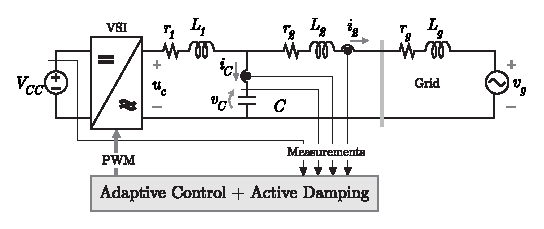
\includegraphics[width=0.9\textwidth]{img/LCL_geral}}
            \def\svgwidth{\textwidth}
            \input{./img/LCL_geral.pdf_tex}}
        \renewcommand\figurename{Fig.}
        \caption{Filtro LCL para o caso monofásico.}
        \label{fig:LCL_geral}
    \end{figure}

    Visto que a transformação (\ref{eq:alpha_beta_0}) é invariante no tempo, ela pode ser
    aplicada ao modelo (\ref{eq:LCL_abc_espaco_estados}). Dessa forma, tem-se que
    %
    \begin{equation}
        \begin{split}
            \mathbf{T}_{\alpha \beta 0} \frac{d}{dt} \mathbf{x}_{abc}(t) & =
                \mathbf{T}_{\alpha \beta 0} \mathbf{A}_{abc} \mathbf{x}_{abc}(t) +
                \mathbf{T}_{\alpha \beta 0} \mathbf{B}_{abc} \mathbf{u}_{abc}(t) +
                \mathbf{T}_{\alpha \beta 0} \mathbf{F}_{abc} \mathbf{v}_{abc}(t) \\
            \mathbf{T}_{\alpha \beta 0} \mathbf{y}_{abc}(t) & = \mathbf{T}_{\alpha \beta 0}
                \mathbf{C}_{abc} \mathbf{x}_{abc}(t) \text{,}
        \end{split}
    \end{equation}
    %
    isto é,
    %
    \begin{equation}
        \begin{split}
            \frac{d}{dt} \mathbf{x}_{\alpha \beta 0}(t) & =
                \mathbf{A}_{\alpha \beta 0} \mathbf{x}_{\alpha \beta 0}(t) +
                \mathbf{B}_{\alpha \beta 0} \mathbf{u}_{\alpha \beta 0}(t) +
                \mathbf{F}_{\alpha \beta 0} \mathbf{v}_{\alpha \beta 0}(t) \\
            \mathbf{y}_{\alpha \beta 0}(t) & = \mathbf{C}_{\alpha \beta 0}
                \mathbf{x}_{\alpha \beta 0}(t) \text{.}
        \end{split}
        \label{eq:LCL_ab0_espaco_estados}
    \end{equation}

    O modelo (\ref{eq:LCL_ab0_espaco_estados}) representa o sistema na forma de dois
    sistemas monofásicos desacoplados associados ao eixo $\alpha$ e ao eixo $\beta$. O
    eixo $0$ pode ser desconsiderado, já que não há caminho para circulação de corrente
    de sequência zero.

\section{Modelo em Função de Transferência}

    Uma forma conveniente de modelar o sistema é através de impedâncias
    complexas~\cite{ref:XU}. As indutâncias e a capacitância do filtro podem ser
    representadas pelas seguintes impedâncias
    %
    \begin{equation}
        \begin{split}
            Z_i & = r_1 + L_1 s \text{,} \\
            Z_C & = \frac{1}{s C} \text{,} \\
            Z_g & = r_2 + r_g + \left( L_2 + L_g \right) s \text{.}
        \end{split}
    \end{equation}

    A impedância do lado da rede $Z_g$ engloba duas indutâncias: uma indutância projetada,
    $L_2$, e uma indutância desconhecida que é a indutância da rede elétrica $L_g$. Escolheu-se
    essa forma de representação de modo a explicitar a incerteza paramétrica, apesar de $L_2$
    ser uma indutância projetada. Além disso, é importante esclarecer que a tensão da rede
    $v_g$ pode ser desprezada na obtenção do modelo, visto que é um distúrbio exógeno que
    deve ser rejeitado pelo controlador adaptativo.

    % A Fig.~\ref{fig:estrutura_geral_cascata} demonstra a estrutura de controle utilizada.

    % \begin{figure}[htb]
    %     \centering{
    %         %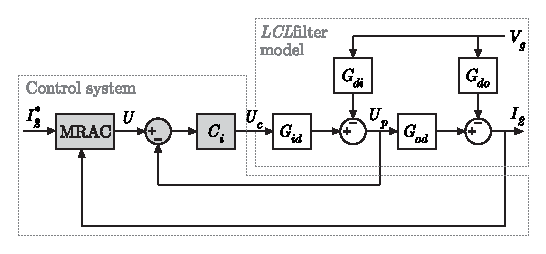
\includegraphics[width=0.9\textwidth]{img/cascade_general}}
    %         \def\svgwidth{0.9\textwidth}
    %         \input{./img/multiloop_geral.pdf_tex}}
    %     \renewcommand\figurename{Fig.}
    %     \caption{Diagrama de blocos demonstrando a estrutura geral de controle.}
    %     \label{fig:estrutura_geral_cascata}
    % \end{figure}

    % Observa-se que $U_p$ indica a variável de controle intermediária utilizada para
    % implementar a malha interna e realizar o amortecimento ativo da ressonância do filtro,
    % podendo ser $V_C$ ou $I_C$. O controlador adaptativo na malha externa gera a referência
    % $U$ para a malha interna, que por sua vez gera a ação de controle $U_c$ implementada
    % via PWM.

    Considerando a estrutura da Fig.~\ref{fig:LCL_geral} e desprezando o distúrbio da
    rede $v_g$, obtém-se as seguintes expressões a partir das leis de Kirchhoff
    %
    \begin{equation}
        \frac{V_C}{U_c} = \frac{Z_C Z_g}{Z_i \left( Z_C + Z_g \right) + Z_C Z_g}
        \text{,}
        \label{eq:vc_uc}
    \end{equation}
    %
    \begin{equation}
        \frac{I_C}{U_c} = \frac{Z_g}{Z_i \left( Z_C + Z_g \right) + Z_C Z_g}
        \text{,}
        \label{eq:ic_uc}
    \end{equation}
    %
    \begin{equation}
        \frac{I_2}{U_c} = \frac{Z_C}{Z_i \left( Z_C + Z_g \right) + Z_C Z_g}
        \text{.}
    \end{equation}

    Do ponto de vista de amortecimento ativo, todo e qualquer elemento resistivo
    que se encontre no sistema irá colaborar com o amortecimento, embora de forma
    passiva. Por esse motivo, as resistências são desprezadas na modelagem do
    sistema, visto que isto irá facilitar a modelagem e criar um caso pior do que
    o que se encontra na prática.

    A discretização destas funções de transferência é feita conforme realizado
    em \cite{ref:PARKER}, incluindo um retentor de ordem zero (ZOH) e aplicando a
    transformada $\mathcal{Z}$. Dessa forma, considerando o atraso de tempo associado
    à implementação digital, obtém-se
    %
    \begin{equation}
        G_d (z) = \frac{I_2}{U_c} = K_1 \frac{1}{z \left( z-1 \right)}
        - \frac{K_1 \sen \left( \omega_n T_s \right) }{\omega_n T_s}
        \frac{z-1}{z \left( z^2 - 2 \cos\left( \omega_n T_s \right) z +1 \right) }
        \text{,}
    \end{equation}
    %
    onde $T_s$ é o período de amostragem e
    %
    \begin{equation}
        K_1 = \frac{T_s}{L1 + L2 + Lg} \text{,}
    \end{equation}
    %
    \begin{equation}
        \omega_n = \sqrt{\frac{ L_1 + L_2 + L_g }{ L_1 C \left( L_2 + L_g \right)}}
        \text{.}
    \end{equation}

    No caso em que a variável intermediária é a tensão do capacitor $V_C$, para
    relacionar $I_2$ com $V_C$ é necessário discretizar a equação~(\ref{eq:vc_uc})
    %
    \begin{equation}
        G_{id}(z) = \frac{2 \sen^2 \left( \omega_n \frac{T_s}{2} \right)}{L_1 C \omega_n^2}
            \frac{z+1}{z \left( z^2 - \cos \left( \omega_n T_s \right) z + 1 \right)}
            \text{.}
    \end{equation}

    Dessa forma, a relação $G_{od}$ entre $I_2$ e $V_C$ é
    %
    \begin{equation}
        G_{od}(z) = \frac{I_2}{V_C} = \frac{G_d}{G_{id}} \text{.}
    \end{equation}

    De forma semelhante, no caso em que a variável intermediária é a corrente do
    capacitor $I_C$, para relacionar $I_2$ com $I_C$ é necessário discretizar a
    equação~(\ref{eq:ic_uc})
    %
    \begin{equation}
        G_{id}(z) = \frac{\sen \left( \omega_n T_s \right)}{\omega_n L_1}
            \frac{z-1}{z \left( z^2 - \cos \left( \omega_n T_s \right) z + 1 \right)}
            \text{,}
    \end{equation}
    %
    e assim
    %
    \begin{equation}
        G_{od}(z) = \frac{I_2}{I_C} = \frac{G_d}{G_{id}} \text{.}
    \end{equation}


%FIM---------------------------------------------------------------------------
